\documentclass{standalone}

\usepackage{tikz}
\usepackage{amsmath,mathtools}

\usepackage{pgfplots}
\usepackage{amsmath,amsthm}
\usepackage{subcaption} 
\usepackage{xspace}
\usepackage{threeparttable}  % For \begin{tablenotes}
\usepackage{multirow}
\usepackage{xcolor}
% Math & symbols


% Units like \SI{10}{m/s}
\usepackage{siunitx}

% Tables
\usepackage{booktabs}

% Figures
\usepackage{graphicx}
\usepackage{subcaption}   % for subfigures

% Floats (for [H] in algorithm)
\usepackage{float}


\usepackage{algorithm}
\usepackage{algpseudocode} % provides algorithmicx/algpseudocode

% Lists (for custom labels S1, S2, …)
\usepackage{enumitem}

\usepackage{multirow}


\usepackage[T1]{fontenc}
\usepackage[tt=false,type1=true]{libertine} % match acmart’s Libertine options
\usepackage[varqu]{zi4}                    % match acmart’s mono setup
\usepackage[libertine]{newtxmath}          % match acmart math (incl. \mathcal)
\def\mathdefault#1{#1}


\AtBeginDocument{%
  \providecommand\BibTeX{{%
    Bib\TeX}}}


\newcommand{\revisionColor}{black}

\usetikzlibrary{intersections, patterns}
\usepgfplotslibrary{groupplots}
\pgfplotsset{compat=1.18}


\usetikzlibrary{positioning}
\usetikzlibrary{ arrows.meta}
\usetikzlibrary{shapes.geometric}
\usetikzlibrary{calc}
\usetikzlibrary{arrows}
\usetikzlibrary{shapes, arrows, positioning, fit, calc, backgrounds, chains,decorations.pathreplacing,hobby}
\usetikzlibrary{mindmap,trees}
\usetikzlibrary{automata,positioning}
\usetikzlibrary{decorations.markings}





\def\distanceXToDT{19}
\def\distanceYToDT{0.4}
\def\distanceL{0.9}
\def\distance2L{2}
\def\innersep{0.4}
\def\squareHeight{0.5}
\def\squareWidth{1.2}
\def\BigSquareWidth{0.4\textwidth}

\def\viewFont{\scriptsize}

\tikzset{% UML2 Activity Diagram Styles
  pin/.style    = {fill=white,draw, thin, rectangle, minimum height = 0.4em,
    minimum width = 0.4em, node distance=-1pt, inner sep=0},
  pin left triangle/.style = {pin,append after command={
      \pgfextra{
        \draw[fill=black] 
          (\tikzlastnode.south east) -- (\tikzlastnode.north east) -- 
          ([xshift=-0.4em]\tikzlastnode.east) -- cycle;
      }
    }
  },
  pin up triangle/.style = {
    pin,
    path picture={
      \draw[fill=white, draw=black, thin]
        ([xshift=-0.3em,yshift=-0.3em]path picture bounding box.center) --
        ([xshift=0.3em,yshift=-0.3em]path picture bounding box.center) --
        ([yshift=0.3em]path picture bounding box.center) -- cycle;
    },
  },
  pin left triangle/.style = {
    pin,
    path picture={
      \draw[fill=black, draw=black]
        ([xshift=0.3em,yshift=-0.3em]path picture bounding box.center) --
        ([xshift=0.3em,yshift=0.3em]path picture bounding box.center) --
        ([xshift=-0.3em]path picture bounding box.center) -- cycle;
    },
  },
  pin right triangle/.style = {
    pin,
    path picture={
      \draw[fill=black, draw=black]
        ([xshift=-0.3em,yshift=-0.3em]path picture bounding box.center) --
        ([xshift=-0.3em,yshift=0.3em]path picture bounding box.center) --
        ([xshift=0.3em]path picture bounding box.center) -- cycle;
    },
  },
  view/.style    = {draw, rectangle, dashed,  minimum width=\squareWidth cm, minimum height=\squareHeight cm },
}

\begin{document}

      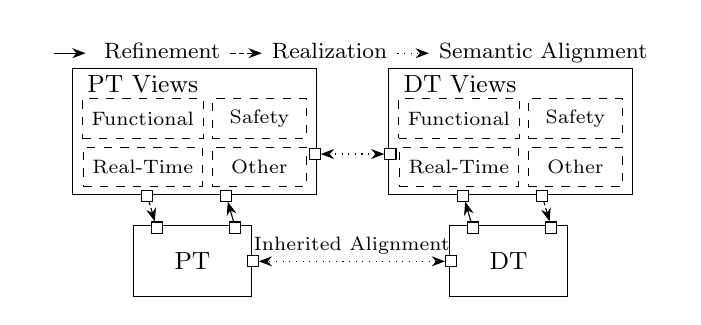
\begin{tikzpicture}[node distance=3cm, font = \small, >=Stealth]
      

      \node[draw, rectangle,
       minimum height=0.9cm,
      align=center, minimum width=1.5cm] (Deployed) at (0,0)
      {PT};

      
    
      
      % System Views
      \node[view, above= 1.1 cm of Deployed, xshift=0.85cm] (PTS) {\viewFont Safety};
     \node[view, below = 0.1 cm of PTS] (PTO) {\viewFont Other};
     \node[view, left = 0.1 cm of PTS] (PTF) {\viewFont Functional};

     \node[view,below = 0.1 cm of PTF] (PTR) {\viewFont Real-Time};
      \node[draw,rectangle, minimum width=3cm,minimum height=1.6cm,fit={(PTF)(PTS)(PTR)(PTO)},yshift=4pt,  label={[anchor=north west, xshift=2pt, yshift=1pt]north west:PT Views}] (PTV) {};


        \node[draw, rectangle,
       minimum height=0.9cm,
      align=center, right = 2.5cm of Deployed, minimum width=1.5cm] (Proposed)
      {DT};

    % Virtual  Views
      \node[view, above= 1.1 cm of Proposed, xshift = 0.85cm] (DTS) {\viewFont Safety};
     \node[view, below = 0.1 cm of DTS] (DTO) {\viewFont Other};
     \node[view, left = 0.1 cm of DTS] (DTF) {\viewFont Functional};

     \node[view,below = 0.1 cm of DTF] (DTR) {\viewFont Real-Time};

      \node[draw,rectangle, minimum width=3cm, minimum height=1.6cm,fit={(DTF)(DTS)(DTR)(DTO)},yshift=4pt,  label={[anchor=north west, xshift=2pt, yshift=1pt]north west:DT  Views}] (DTV) {};



      \node [pin ,left=of DTV, xshift=0.2 em, yshift= -0.285cm](plDTV){};
      \node [pin ,right=of PTV, xshift=-0.2 em, yshift= -0.285cm](prPTV){};
      \draw[<->, dotted] (plDTV) -- (prPTV);



      \node [pin ,below=of PTV, yshift=0.1 em, xshift= 0.4cm](pbPTV){};
      \node [pin ,below=of PTV, yshift=0.1 em, xshift= -0.6cm](pbPTV2){};
      \node [pin ,above=of Deployed, yshift=-0.2 em, xshift= 0.544cm](puDeployed){};
      \node [pin ,above=of Deployed, yshift=-0.2 em, xshift= -0.455cm](puDeployed2){};

      \draw[->] (puDeployed)--(pbPTV) ;
      \draw[<-, dash pattern=on 2pt off 1pt] (puDeployed2) -- (pbPTV2);

      
      \node [pin ,below=of DTV, yshift=0.1 em, xshift= -0.6cm](pbDTV){};
      \node [pin ,below=of DTV, yshift=0.1 em, xshift= 0.4cm](pbDTV2){};
      \node [pin ,above=of Proposed, yshift=- 0.2 em, xshift=-0.455cm](puProposed){};
      \node [pin ,above=of Proposed, yshift=- 0.2 em, xshift=0.544cm](puProposed2){};
      \draw[->]  (puProposed) -- (pbDTV);
      \draw[<-, dash pattern=on 2pt off 1pt] (puProposed2) -- (pbDTV2);

      
      \node [pin ,left=of Proposed, xshift=0.2em](plProposed){};
      
      \node [pin ,right=of Deployed, xshift=- 0.1 em](prDeployed){};
      %\draw[->] (plProposed) -- (prDeployed);

      \node [pin ,right=of Deployed, xshift=- 0.1 em](prDeployed){};
      \draw[<->,dotted] (plProposed) -- node[above, yshift=-0.1em, font=\scriptsize]{Inherited Alignment} (prDeployed);

      % Monitoring & adaptation loop (dotted, curved)
%\draw[dotted, <->] (plProposed) to[bend right=35]    node[above, yshift=-0.3em, font=\scriptsize]{Monitor \& Adaptation} (prDeployed);
      \node at ([yshift=2.2cm]$ (Proposed.north)!0.5!(Deployed.north)$) (Legend) {
  \begin{tabular}{rlrlrl}
    \tikz{\draw[->] (0,0) -- (0.4,0);} &\hspace{-0.3cm} \footnotesize Refinement  & \hspace{-0.3cm}\tikz{\draw[->, dash pattern=on 2pt off 1pt] (0,0) -- (0.4,0);} & \hspace{-0.3cm}\footnotesize Realization
    & \hspace{-0.3cm}\tikz{\draw[->, dotted] (0,0) -- (0.4,0);} & \hspace{-0.3cm}\footnotesize Semantic Alignment

  \end{tabular}
};
%      \draw[->] ([xshift=0.3cm,yshift = 0.2cm]OCM.east) -- ([xshift=0.3cm,yshift=1.3cm]OCM.east);
\end{tikzpicture}
\end{document}

